
% Inbuilt themes in beamer
\documentclass[aspectratio=169]{beamer}
\usepackage{graphicx}
% Theme choice:
\usetheme{CambridgeUS}

% Title page details: 
\title{Econometrics Discussion Section 2} 
\author{John Green}
\date{Spring 2024}


\begin{document}

% Title page
\begin{frame}
    \titlepage 
\end{frame}

% Outline frame
\begin{frame}{Linear regression}
    We now want to move on to examining how to understand the relationship between two variables.
    \begin{itemize}
        \item Distinguish \textit{prediction} from \textit{causation}
        \item Linear regression model
        \item $R^2$, SER, F-test
        \item Necessary assumptions
    \end{itemize}
\end{frame}

\begin{frame}{Minimizing error with one variable}
    \begin{itemize}
        \item Suppose we have data $X_1, X_2, X_3, \ldots, X_n = \{ X_i \}_{i \leq n} $
        \item What is the best guess for the value of an arbitrary $X_j$?
        \begin{itemize}
            \item The best fit will be the mean, $ E[X] $
        \end{itemize}
        \item But wait: which error are we minimizing?
    \end{itemize}
\end{frame}

\begin{frame}{Minimizing error with two variables}
    \begin{itemize}
        \item Which error are we minimizing?
        \begin{itemize}
            \item Usually the \textit{squared} error --- but not necessarily!
        \end{itemize}
        \item Now what if we have data on two variables:
        $$
        (X_1, Y_1), (X_2, Y_2), \ldots, (X_n, Y_n) = \{ (X_i, Y_i) \}_{i \leq n}
        $$
        \item We want to understand their relationship! Suppose we think that $X$ causes $Y$: then we might want to know what is our best guess for an arbitrary $Y_j$, given its $X_j$?
        \begin{itemize}
            \item $X$ is years of education and $Y$ is income; if I tell you that someone has 12 years of education, what is your best guess for their income?
            \item This will be the \textit{conditional expectation}: $E[Y|X=12]$
        \end{itemize}
    \end{itemize}
\end{frame}

\begin{frame}{Minimizing error with two variables}
    \begin{itemize}
        \item We want to understand their relationship! Suppose we think that $X$ causes $Y$: then we might want to know what is our best guess for an arbitrary $Y_j$, given its $X_j$?
        \begin{itemize}
            \item $X$ is years of education and $Y$ is income; if I tell you that someone has 12 years of education, what is your best guess for their income?
            \item This will be the \textit{conditional expectation}: $E[Y|X=12]$
        \end{itemize}
        \item Let's assume a \textit{linear} relationship:
        $$
        Y_i = \beta_0 + \beta_1 X_i
        $$
        \item Then our problem is simply to draw a line through the 2D data which minimizes the errors
        \begin{itemize}
            \item $\beta_0$ is the intercept, $\beta_1$ is the slope
        \end{itemize}
    \end{itemize}
\end{frame}

\begin{frame}
    \centering
    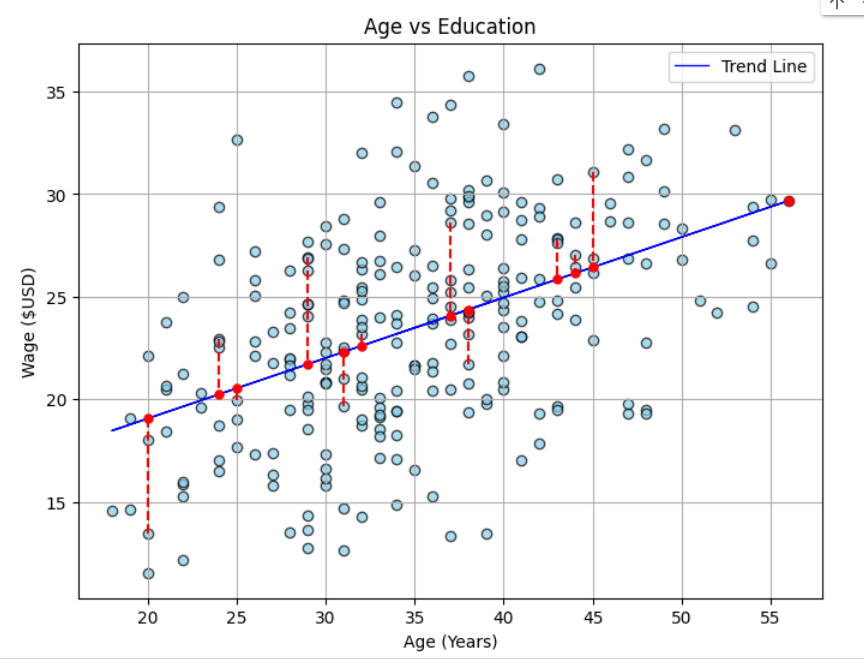
\includegraphics[width = .6\textwidth,keepaspectratio]{./figs/age_ed.png}
\end{frame}

\begin{frame}{Ordinary least squares}
    \begin{itemize}
        \item The line which minimizes the errors is the \textit{ordinary least squares} regression line
        \item Found by solving 
        $$
        \min_{\beta_0, \beta_1} \sum_{i=1}^n (Y_i - (\beta_0 - \beta_1 X_i))^2
        $$
        \item In practice, we only have a \textbf{sample}, and so we have to estimate these two parameters:
        \begin{itemize}
            \item Add an error term: $Y_i = \beta_0 + \beta_1 X_i + \epsilon_i$
            \item We will denote these estimates as $\hat{\beta}_0$ (intercept) and $\hat{\beta}_1$ (slope)
        \end{itemize}
    \end{itemize}
\end{frame}

\begin{frame}{Regression output}
    \begin{itemize}
        \item $R^2$ measures the variance in $Y$ that is explained by $X$
        \begin{itemize}
            \item $R^2 = \frac{ESS}{TSS}$
        \end{itemize}
        \item Standard error of regression (SER): spread of the residual $\epsilon$
        \item Root mean squared error (RMSE): similar, just calculated with $n$ instead of $n-2$ in the denominator
    \end{itemize}
\end{frame}

\begin{frame}{Assumptions}
    \begin{itemize}
        \item All we've done so far is draw a line --- no assumptions needed!
        \item What if we want to think about $X$ as having a causal effect on $Y$, as in the case of more years of school mechanically leading to a higher income?
        \begin{itemize}
            \item eg if we were to hold all other factors constant (as in a controlled and randomized experiment) what do we expect an extra year of education to do to income?
        \end{itemize}
    \end{itemize}
\end{frame}

\begin{frame}{Assumptions}
    \begin{itemize}
        \item $E[\epsilon | X=x] = 0$ 
        \begin{itemize}
            \item So that $\hat{\beta_1}$ is unbiased estimator
        \end{itemize}
        \item $\{ (X_i, Y_i) \}_{i \leq n}$ are i.i.d. 
        \begin{itemize}
            \item Will give us sampling distributions for coefficient estimates
        \end{itemize}
        \item Large outliers are rare 
                Will give us sampling distributions for coefficient estimates
        \begin{itemize}
            \item OLS is sensitive and our estimate $\hat{\beta}$ might be meaningless otherwise
        \end{itemize}
    \end{itemize}
\end{frame}

\begin{frame}{Sampling distribution of $\hat{\beta}$}
    \begin{itemize}
        \item Just like $\bar{Y}$, $\hat{\beta}$ is a random variable and has a sampling distribution! (Why?)
        \item So, if we want to be able to say something about the relationship between an $X$ and a $Y$ using $\hat{\beta}$, we need to know something about its distribution
        \begin{itemize}
            \item Will allow us to test hypotheses, eg that $\beta_1 = 0$
            \item Will let us construct confidence intervals and indicate uncertainty
        \end{itemize}
        \item Extra assumption on top of the OLS assumptions: that the relationship between $X$ and $Y$ is linear (how might we relax this?)
    \end{itemize}
\end{frame}

\begin{frame}{Hypothesis testing for $\hat{\beta}$}
    \begin{itemize}
        \item Will work in a very similar way to the hypothesis testing we've done for the sample mean
        \begin{itemize}
            \item Variance of $\hat{\beta}$ is decreasing in the sample size and in the variance of $X$
        \end{itemize}
        \item We will construct a t-statistic, $t=\frac{\hat{\beta}-\beta}{SE(\hat{\beta})}$
        \item So we can test if $\beta=0$ (ie if $X$ has no relationship with $Y$), or if $\beta<0$ (ie $X$ has a negative relationship with $Y$)
        \item Can CIs as well
    \end{itemize}
\end{frame}

\begin{frame}{Binary regression}
    \begin{itemize}
        \item Sometimes we have a binary regressor: for example, participation in some program
        \begin{itemize}
            \item Effect of taking a drug
        \end{itemize}
        \item OLS works in the same way but interpretation is a little different:
        \begin{itemize}
            \item $Y_i = \beta_0 + \beta_1 D_i + \epsilon_i$
            \item $\beta_0$ is mean with no treatment
            \item $\beta_0 + \beta_1$ is the mean with treatment
            \item So $\beta_1$ is the average treatment effect
        \end{itemize}
    \end{itemize}
\end{frame}

\begin{frame}{Heteroskedasticity}
    \begin{itemize}
        \item Homoskedasticity: $\epsilon$ has constant variance (doesn't depend on X)
        \item If we assume Homoskedasticity, we can say some stronger things about the OLS
        \begin{itemize}
            \item Gauss-Markov theorem: OLS is the best linear unbiased estimator ie has smallest variance
            \item Simpler formula for the variance of $\hat{\beta}$
        \end{itemize}
        \item What if we assume Homoskedasticity but it's not true?
        \begin{itemize}
            \item SE will be too small (probably) meaning that we are \textit{overconfident} in our inference
        \end{itemize}
        \item If we assume normal errors, we can say some even stronger things
        \item Make strong assumptions, get strong results! These are usually difficult to justify.
    \end{itemize}
\end{frame}

\end{document}